%\documentclass[icelandic]{beamer}

\documentclass[icelandic,a4paper,12pt]{article}
\usepackage{beamerarticle}

\mode<presentation>
{
  \usetheme{boxes}
  % með efnisyfirliti: Szeged, Frankfurt 
  % án efnisyfirlits: Pittsburgh
  % áhugavert: CambridgeUS, Boadilla
  %\setbeamercovered{transparent} %gegnsætt
  \setbeamercovered{invisible}
  }

\usepackage[english,icelandic]{babel}
\usepackage[utf8]{inputenc}
\usepackage{t1enc}
\selectlanguage{icelandic}
\usepackage{graphicx}
\usepackage{amsmath}
\usepackage{amssymb}
\usepackage{mathrsfs}
% \newcommand{\C}{{\mathbb  C}}
% \newcommand{\Z}{{\mathbb Z}}
% \newcommand{\R}{{\mathbb  R}}
% \newcommand{\N}{{\mathbb  N}}
% \newcommand{\Q}{{\mathbb Q}}
\renewcommand{\phi}{\varphi}
\renewcommand{\epsilon}{\varepsilon}

%\usepackage{pgfpages}
% \pgfpagesuselayout{2 on 1}[a4paper,border shrink=5mm]

\def\lecturename{Stærðfræðigreining IB}
\title{\insertlecture}
\author{Benedikt Steinar Magnússon, \href{mailto:bsm@hi.is}{bsm@hi.is}}
\institute
{
  Verkfræði- og náttúruvísindasvið\\
  Háskóli Íslands
}
\subtitle{Stærðfræðigreining IB}
%\subject{\lecturename}

\mode<article>
{
	\usepackage[colorlinks=false,
	pdfauthor={Benedikt Steinar Magnusson},
	pdftitle={IB: Namsefni
	}]{hyperref}
  %\usepackage{times}
  %\usepackage{mathptmx}
  \usepackage[left=1.5cm,right=4cm,top=1.5cm,bottom=3cm]{geometry}
}

% Beamer version theme settings

%\useoutertheme[height=0pt,width=2cm,right]{sidebar}
%\usecolortheme{rose,sidebartab}
%\useinnertheme{circles}
%\usefonttheme[only large]{structurebold}

\setbeamercolor{sidebar right}{bg=black!15}
\setbeamercolor{structure}{fg=blue}
\setbeamercolor{author}{parent=structure}

\setbeamerfont{title}{series=\normalfont,size=\LARGE}
\setbeamerfont{title in sidebar}{series=\bfseries}
\setbeamerfont{author in sidebar}{series=\bfseries}
\setbeamerfont*{item}{series=}
\setbeamerfont{frametitle}{size=}
\setbeamerfont{block title}{size=\small}
\setbeamerfont{subtitle}{size=\normalsize,series=\normalfont}

\defbeamertemplate*{footline}{infolines theme}
 {
   \leavevmode%
   \hbox{%
   \begin{beamercolorbox}[wd=.333333\paperwidth,ht=2.25ex,dp=1ex,center]{author in head/foot}%
   %  \usebeamerfont{author in head/foot}\insertshortauthor~~\beamer@ifempty{\insertshortinstitute}{}{(\insertshortinstitute)}
   \end{beamercolorbox}%
   \begin{beamercolorbox}[wd=.333333\paperwidth,ht=2.25ex,dp=1ex,center]{title in head/foot}%
    % \usebeamerfont{title in head/foot}\insertshorttitle
   \end{beamercolorbox}%
   \begin{beamercolorbox}[wd=.333333\paperwidth,ht=2.25ex,dp=1ex,right]{date in head/foot}%
     %\usebeamerfont{date in head/foot}\insertshortdate{}\hspace*{2em}
     \insertshortlecture.\insertframenumber{} / \insertshortlecture.\inserttotalframenumber\hspace*{2ex} 
   \end{beamercolorbox}}%
   \vskip0pt%
 }
  


\setbeamertemplate{sidebar right}
{
  {\usebeamerfont{title in sidebar}%
    \vskip1.5em%
    \hskip3pt%
    \usebeamercolor[fg]{title in sidebar}%
    \insertshorttitle[width=2cm-6pt,center,respectlinebreaks]\par%
    \vskip1.25em%
  }%
  {%
    \hskip3pt%
    \usebeamercolor[fg]{author in sidebar}%
    \usebeamerfont{author in sidebar}%
    \insertshortauthor[width=2cm-2pt,center,respectlinebreaks]\par%
    \vskip1.25em%
  }%
  \hbox to2cm{\hss\insertlogo\hss}
  \vskip1.25em%
  \insertverticalnavigation{2cm}%
  \vfill
  \hbox to 2cm{\hfill\usebeamerfont{subsection in
      sidebar}\strut\usebeamercolor[fg]{subsection in
      sidebar}\insertshortlecture.\insertframenumber\hskip5pt}%
  \vskip3pt%
}%

\setbeamertemplate{title page}
{
  \vbox{}
  \vskip1em
  %{\huge Kapitel \insertshortlecture\par}
  {\usebeamercolor[fg]{title}\usebeamerfont{title}\inserttitle\par}%
  \ifx\insertsubtitle\@empty%
  \else%
    \vskip0.25em%
    {\usebeamerfont{subtitle}\usebeamercolor[fg]{subtitle}\insertsubtitle\par}%
  \fi%     
  \vskip1em\par
  %Vorlesung \emph{\lecturename}\ vom 
  \insertdate\par
  \vskip0pt plus1filll
  \leftskip=0pt plus1fill\insertauthor\par
  \insertinstitute\vskip1em
}

%\logo{\includegraphics[width=2cm]{beamerexample-lecture-logo.pdf}}



% Article version layout settings

\mode<article>

\makeatletter
\def\@listI{\leftmargin\leftmargini
  \parsep 0pt
  \topsep 5\p@   \@plus3\p@ \@minus5\p@
  \itemsep0pt}
\let\@listi=\@listI


\setbeamertemplate{frametitle}{\paragraph*{\insertframetitle\
    \ \small\insertframesubtitle}\ \par
}
\setbeamertemplate{frame end}{%
  \marginpar{\scriptsize\hbox to 1cm{\sffamily%
      \hfill\strut\insertshortlecture.\insertframenumber}\hrule height .2pt}}
\setlength{\marginparwidth}{1cm}
\setlength{\marginparsep}{1.5cm}

\def\@maketitle{\makechapter}

\def\makechapter{
  \newpage
  \null
  \vskip 2em%
  {%
    \parindent=0pt
    \raggedright
    \sffamily
    \vskip8pt
    %{\fontsize{36pt}{36pt}\selectfont Kapitel \insertshortlecture \par\vskip2pt}
    {\fontsize{24pt}{28pt}\selectfont \color{blue!50!black} \insertlecture\par\vskip4pt}
    {\Large\selectfont \color{blue!50!black} \insertsubtitle, \@date\par}
    \vskip10pt

    \normalsize\selectfont \@author\par\vskip1.5em
    %\hfill BLABLA
  }
  \par
  \vskip 1.5em%
}

\let\origstartsection=\@startsection
\def\@startsection#1#2#3#4#5#6{%
  \origstartsection{#1}{#2}{#3}{#4}{#5}{#6\normalfont\sffamily\color{blue!50!black}\selectfont}}

\makeatother

\mode
<all>




% Typesetting Listings

\usepackage{listings}
\lstset{language=Java}

\alt<presentation>
{\lstset{%
  basicstyle=\footnotesize\ttfamily,
  commentstyle=\slshape\color{green!50!black},
  keywordstyle=\bfseries\color{blue!50!black},
  identifierstyle=\color{blue},
  stringstyle=\color{orange},
  escapechar=\#,
  emphstyle=\color{red}}
}
{
  \lstset{%
    basicstyle=\ttfamily,
    keywordstyle=\bfseries,
    commentstyle=\itshape,
    escapechar=\#,
    emphstyle=\bfseries\color{red}
  }
}



% Common theorem-like environments

\theoremstyle{definition}
\newtheorem{exercise}[theorem]{\translate{Exercise}}




% New useful definitions:

\newbox\mytempbox
\newdimen\mytempdimen

\newcommand\includegraphicscopyright[3][]{%
  \leavevmode\vbox{\vskip3pt\raggedright\setbox\mytempbox=\hbox{\includegraphics[#1]{#2}}%
    \mytempdimen=\wd\mytempbox\box\mytempbox\par\vskip1pt%
    \fontsize{3}{3.5}\selectfont{\color{black!25}{\vbox{\hsize=\mytempdimen#3}}}\vskip3pt%
}}

\newenvironment{colortabular}[1]{\medskip\rowcolors[]{1}{blue!20}{blue!10}\tabular{#1}\rowcolor{blue!40}}{\endtabular\medskip}

\def\equad{\leavevmode\hbox{}\quad}

\newenvironment{greencolortabular}[1]
{\medskip\rowcolors[]{1}{green!50!black!20}{green!50!black!10}%
  \tabular{#1}\rowcolor{green!50!black!40}}%
{\endtabular\medskip}



\lecture[1]{2. Markgildi og samfelldni}{lecture-text}
\date{29. ágúst 2015}

\newcommand{\C}{{\mathbb  C}}
\newcommand{\Z}{{\mathbb Z}}
\newcommand{\R}{{\mathbb  R}}
\newcommand{\N}{{\mathbb  N}}
\newcommand{\Q}{{\mathbb Q}}
\newcommand{\Sin}{{\text{Sin}}}
\newcommand{\Tan}{{\text{Tan}}}
\newcommand{\Cos}{{\text{Cos}}}
\newcommand{\Cosh}{{\text{Cosh}}}
\newcommand{\arsinh}{{\text{arsinh}}}
\newcommand{\arcosh}{{\text{arcosh}}}
\newcommand{\artanh}{{\text{artanh}}}


\begin{document}
\setcounter{tocdepth}{2}
\tableofcontents

\section{Torræð föll}
\subsection{Náttúrlegi logrinn}
\subsubsection{Skilgreining: Náttúrlegi logrinn}
Látum $A_{x_0}$ tákna flatarmál svæðisins sem
afmarkast af $x$-ás, grafinu $y=\frac{1}{x}$ og línunum $x=1$ og
$x=x_0$.
\pause
Þá skilgreinum við \emph{náttúrlega logrann} með
formúlunni 
\begin{equation*}
\ln x =\left\{\begin{array}{ll}
A_x & \mbox{ef }x\geq 1,\\
-A_x & \mbox{ef }0<x<1.
\end{array}
\right.
\end{equation*}

%GeoGebra
\pause
\subsubsection{Setning}  
$$
\frac{d}{dx}\ln x=\frac{1}{x}.
$$

\subsubsection{Setning}
Fyrir allar tölur $x,y>0$ gildir að:\pause
\begin{enumerate}[(i)]
\item $\ln(1) = 0$\pause
\item  $\ln(xy)=\ln x+\ln y$\pause
\item  $\ln(1/x)=-\ln x$\pause
\item  $\ln(x/y)=\ln x-\ln y$\pause
\item $\ln (x^r)=r\ln x$. 
\end{enumerate}
 
\subsection{Veldisvísisfallið}
\subsubsection{Setning}
Fallið $\ln x$ er strangt vaxandi og þar með eintækt.

\pause

\subsubsection{Skilgreining: Veldisvísisfallið}
Fallið $\exp x$ er skilgreint sem andhverfa fallsins $\ln x$.
\pause
Skilgreiningarsvæði  $\exp x$ er jafnt myndmengi $\ln x$ sem er $\R$.
\pause
Myndmengi $\exp x$ er jafnt skilgreiningarsvæði $\ln x$ sem er bilið
$(0,\infty)$.  

\begin{center}
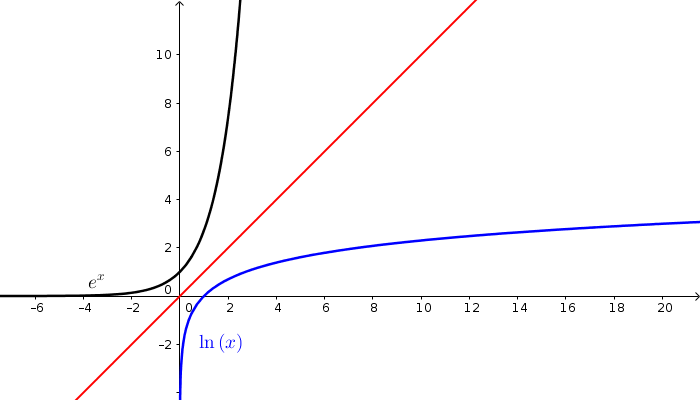
\includegraphics[width=5cm,keepaspectratio=true]{./myndir/kafli04/02_ln-exp.png}
\end{center}

\subsubsection{Skilgreining: Talan $e$}
Skilgreinum töluna með $e=\exp 1$. 

\pause

Það þýðir að $\ln(e)=1$, \pause og talan $e$ 
ákvarðast þess vegna af því að flatarmál svæðisins milli $x$-ás og
grafs $\frac 1x$ á bilinu $[1,e]$ sé 1.
 
\begin{center}
 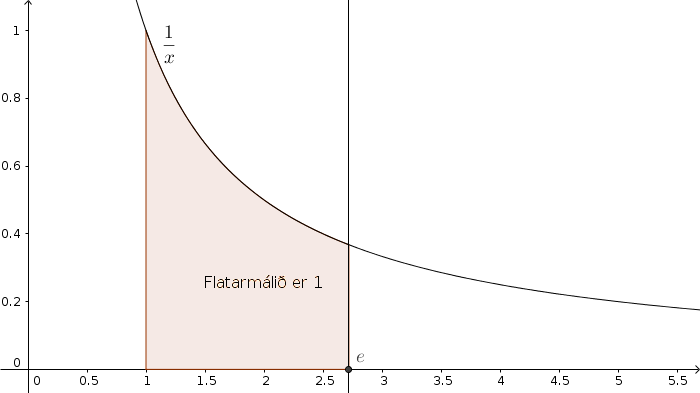
\includegraphics[width=7cm,keepaspectratio=true]{./myndir/kafli04/02_ln-e.png}
\end{center}


% Mynd / Geogebra

 \subsubsection{Setning}
\textbf{Hver er munurinn á $e^x$ eða $\exp x$?}

$e^x$ er aðeins skilgreint þegar $x$ er ræð tala, en $\exp(x)$ er skilgreint 
fyrir allar rauntölur því $\ln:(0,\infty)\to \R$ er átæk.

Það er hins vegar hægt að sýna að 
 $$
 \exp x=\lim_{r\rightarrow x \mbox{\scriptsize\ ($r$ ræð tala)}}e^r
 $$

\pause 

Því er eðlilegt að rita fyrir rauntölu $x$, hvort sem hún er ræð
 eða óræð, að $e^x=\exp x$. 
\pause 
Þannig að héðan í frá gerum við engan
greinarmun á $e^x$ og $\exp x$, við notum bara það sem
lítur betur út fagurfræðilega.


\pause

\subsubsection{Athugasemd}
Athugið að 
$$e^{\ln x}=x \mbox{ fyrir allar tölur }x>0\qquad \mbox{og}\pause
\qquad \ln(e^x)=x  \mbox{ fyrir allar tölur }x.$$



\subsubsection{Eiginleikar veldisvísisfallsins}
Út frá eiginleikum lograns fáum við svo eftirfarandi

\begin{enumerate}[(i)]
\item  $e^0=1$
\item  $e^{x+y}=e^x e^y$
\item  $e^{-x}=\frac{1}{e^x}$
\item  $e^{x-y}=\frac{e^x}{e^y}$
\item  $\left(e^x\right)^y=e^{xy}$
\end{enumerate}


\subsubsection{Athugasemd}
\textbf{Hænan eða eggið?}
Hér höfum við nálgast $\ln$ og $\exp$ þannig að 
við byrjum á að skilgreina $\ln$ með heildi (flatarmáli) og
finnum svo andhverfu lograns, $\exp$. 

\pause

Einnig væri mögulegt að byrja á því að sýna að $e^x$ sé 
vel skilgreint, ekki bara fyrir ræð $x$ heldur einnig 
óræð. Það myndum við gera með því að nota markgildið
$$\lim_{r\rightarrow x \mbox{\scriptsize\ ($r$ ræð tala)}}e^r,$$
hér að ofan, og taka þá $e^x$ sem skilgreiningu á 
$\exp x$ og finna svo andhverfuna, $\ln$.

\pause

Báðar þessar aðferðir hafa kosti og galla, en við notum þá
fyrri vegna þess hvað hún gefur myndræna framsetningu á 
logranum.
 
\subsection{Önnur veldisvísisföll og lograr}
\subsubsection{Skilgreining}
Fyrir tölu $a>0$ og rauntölu $x$ skilgreinum við 
$$a^x=e^{x\ln a}.$$

\subsubsection{Skilgreining}
Andhverfa fallsins $a^x$ er kölluð \emph{logri með grunntölu $a$} og
táknuð með $\log_a x$.  Fallið   $\log_a x$ er skilgreint fyrir öll
$x>0$.

\subsubsection{Athugasemd}
$$y
=\log_a(x)\qquad \text{ þá og því aðeins að } \qquad x = a^y.
$$

\subsubsection{Setning}
Fyrir rauntölu $a>0$ og allar rauntölur $x,y$ gildir að:

\begin{enumerate}[(i)]
\item $a^0=1$
\item $a^1=a$
\item $a^{x+y}=a^xa^y$
\item $a^{-x}=\frac{1}{a^x}$
\item $a^{x-y}=\frac{a^x}{a^y}$
\item $\big(a^x\big)^y=a^{xy}$
\item $(ab)^x=a^xb^x$ (hér er forsenda að $b>0$).
\end{enumerate}

Fyrir rauntölu $a>0$ og allar rauntölur $x,y$ gildir að:
\begin{enumerate}[(i)]
\item $\log_a 1=0$
\item $\log_a a = 1$
\item $\log_a(xy)=\log_a x+\log_a y$
\item $\log_a (1/x)=-\log_a x$
\item $\log_a (x/y)=\log_a x-\log_a y$
\item $\log_a (x^y)=y\log_a x$
\item $\log_a x=\frac{\log_b x}{\log_b a}$ (hér er forsenda að $b>0$).
\end{enumerate}

\subsection{Eiginleikar veldisvísisfalla og logra}
\subsubsection{Setning}
\begin{enumerate}[(i)]
\item  $\frac{d}{dx}\ln x=\frac 1x$\pause
\item  $\frac{d}{dx}e^x=e^x$\pause
\item  $\frac{d}{dx}a^x=(\ln a)a^x$\pause
\item  $\frac{d}{dx}\log_a x=\frac{1}{(\ln a)x}$
\end{enumerate}

\subsubsection{Setning}
Ef $a>0$ þá er 
\begin{enumerate}[(i)]
\item $\lim_{x\to \infty} \frac{x^a}{e^x} = 0$
\item $\lim_{x\to \infty} \frac{\ln(x)}{x^a} = 0$
\item $\lim_{x\to -\infty} |x|^a e^x = 0$
\item $\lim_{x\to 0^+} x^a\, \ln(x) = 0$
\end{enumerate}		

\subsubsection{Athugasemd}
Athugið að setningin að ofan gildir óháð því hversu
stórt $a$ er ((a) og (c) liður) eða hversu lítið
$a$ er ((b) og (d) liður).

\subsubsection{Með öðrum orðum}
Þegar veldi og veldisvísisfall kljást, þá vinnur veldisvísisfallið.

Þegar veldi og logri kljást, þá vinnur veldið.

\subsection{Andhverfur hornafalla}

\subsubsection{Andhverfa $\sin$}
Fallið $\sin(x)$ skilgreint á öllum rauntalnaásnum er ekki 
eintækt og á sér því ekki andhverfu. 

Við getum hins vegar takmarkað okkur við hálfa lotu, þ.e.~skoðum
bara $x\in [-\frac \pi 2, \frac \pi 2]$. \pause $\sin(x)$ takmarkað 
við þetta bil táknum við með $\Sin(x)$. \pause $\Sin$ er strangt 
vaxandi og því eintækt á þessu bili, og hefur þar af leiðandi andhverfu.

\pause

\subsubsection{Skilgreining: $\arcsin$}
\emph{Andhverfa sínussins}, táknuð $\arcsin(x)$ (eða $\sin^{-1}(x)$), 
er andhverfa $\Sin$ og hefur því myndmengið $[-\frac \pi 2, 
\frac \pi 2]$ og skilgreiningarmengið $[-1,1]$.
 
\begin{center}
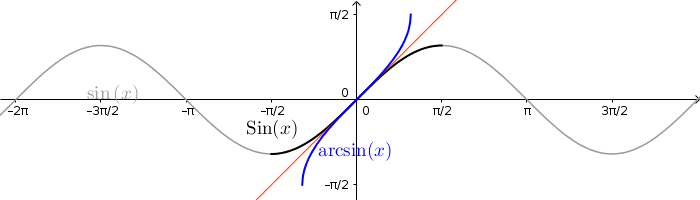
\includegraphics[width=11cm,keepaspectratio=true]{./myndir/kafli04/05_arcsin.png}
\end{center}

\subsubsection{Andhverfa $\cos$}
Fallið $\cos(x)$ skilgreint á öllum rauntalnaásnum er ekki 
eintækt og á sér því ekki andhverfu. 

\pause

Við getum hins vegar takmarkað okkur við hálfa lotu, þ.e.~skoðum
bara $x\in [0, \pi]$. \pause $\cos(x)$ takmarkað 
við þetta bil táknum við með $\Cos(x)$. \pause $\Cos$ er strangt 
minnkandi og því eintækt á þessu bili, og hefur þar af leiðandi andhverfu.

\pause

\subsubsection{Skilgreining: $\arccos$}
\emph{Andhverfa kósínussins}, táknuð $\arccos(x)$ (eða $\cos^{-1}(x)$), 
er andhverfa $\Cos$ og hefur því myndmengið $[0,\pi]$ 
og skilgreiningarmengið $[-1,1]$.
 
\begin{center}
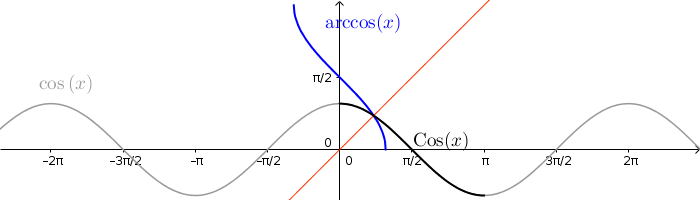
\includegraphics[width=11cm,keepaspectratio=true]{./myndir/kafli04/05_arccos.png}
\end{center}

\subsubsection{Andhverfa tangens}
Fallið $\tan(x) = \frac{\sin(x)}{\cos(x)}$ skilgreint á 
$\{x \in \R; x \neq \pi k + \frac \pi 2, k \in \Z \}$ er ekki 
eintækt og á sér því ekki andhverfu. 

\pause

Við getum hins vegar takmarkað okkur við eina lotu, þ.e.~skoðum
bara $x\in (-\frac \pi 2, \frac \pi 2)$. \pause Athugið
að hér eru endapunktar bilsins ekki með. \pause $\tan(x)$ takmarkað 
við þetta bil táknum við með $\Tan(x)$. \pause $\Tan$ er strangt 
vaxandi og því eintækt á þessu bili, og hefur þar af leiðandi andhverfu.

\pause

\subsubsection{Skilgreining: $\arctan$}
\emph{Andhverfa tangensins}, táknuð $\arctan(x)$ (eða $\tan^{-1}(x)$), 
er andhverfa $\Tan$ og hefur því myndmengið $(-\frac \pi 2,
\frac \pi 2)$ 
og skilgreiningarmengið $(-\infty,\infty)$. \pause Þar að auki
þá er \\
$\lim_{x\to \infty} \arctan(x) = \frac \pi 2$ og \\
$\lim_{x\to -\infty} \arctan(x) = -\frac \pi 2$.
 
\begin{center}
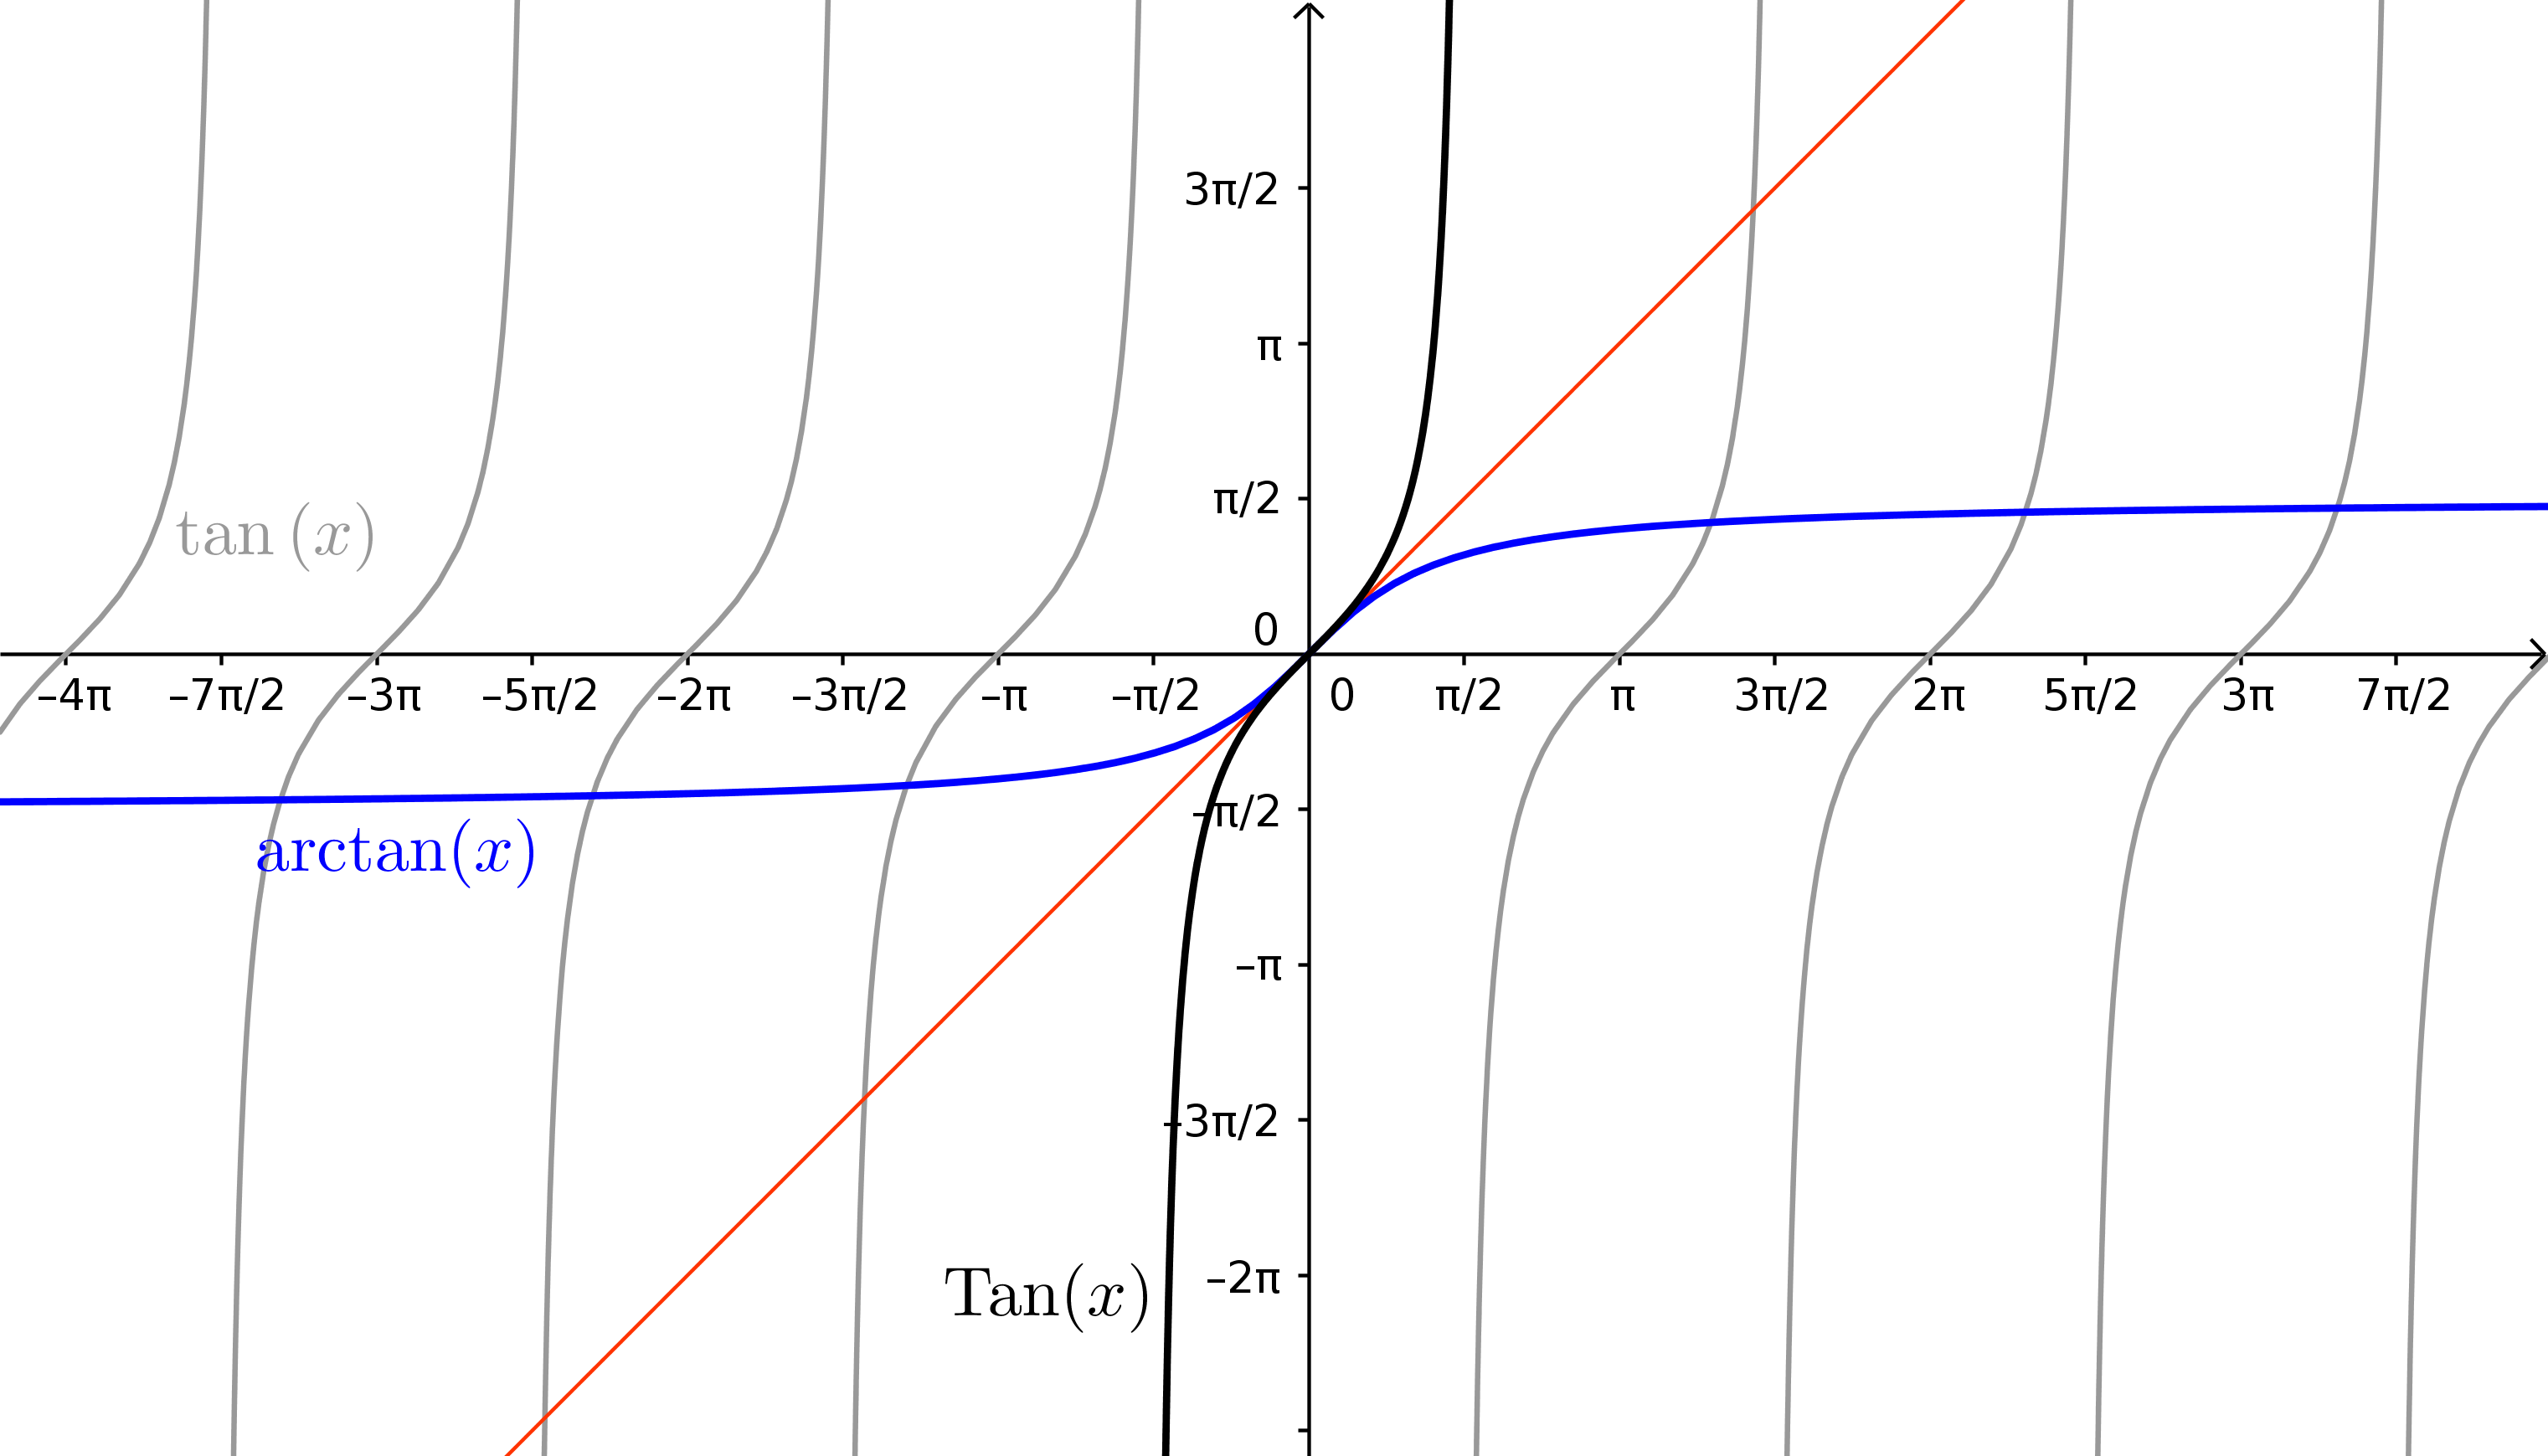
\includegraphics[width=11cm,keepaspectratio=true]{./myndir/kafli04/05_arctan.png}
\end{center}

\subsubsection{Setning}
\begin{enumerate}[(i)]
\item $\frac d{dx} \arcsin(x) = \frac 1{\sqrt{1-x^2}}$ \pause
\item $\frac d{dx} \arccos(x) = \frac {-1}{\sqrt{1-x^2}}$ \pause
\item $\frac d{dx} \arctan(x) = \frac 1{1+x^2}$ 
\end{enumerate}

\subsection{Breiðbogaföll}
\subsubsection{Skilgreining}
Við skilgreinum \emph{breiðbogasínus}, $\sinh$, og 
\emph{breiðbogakósínus},
$\cosh$, með eftirfarandi formúlum  \pause
\begin{eqnarray*}
\sinh(x) &= \frac{e^x - e^{-x}}2,\\ \pause
\cosh(x) &= \frac{e^x + e^{-x}}2.
\end{eqnarray*}
 
\begin{center}
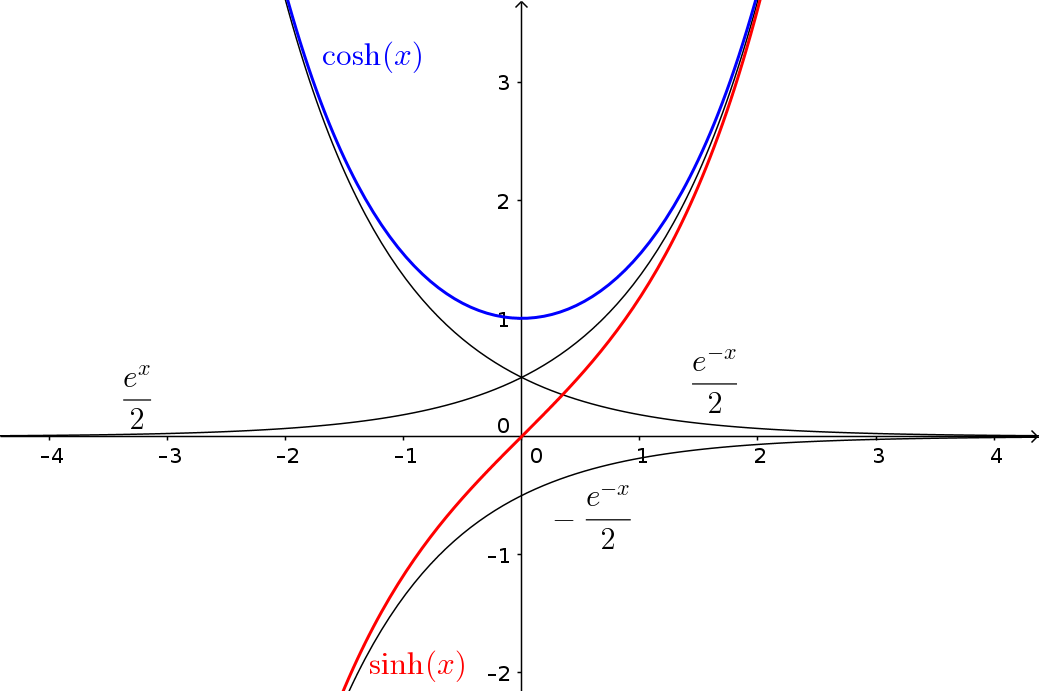
\includegraphics[width=10cm,keepaspectratio=true]{./myndir/kafli04/06_sinh-cosh.png}
\end{center}

\subsubsection{Setning}
\begin{enumerate}[(i)]
\item $\frac d{dx} \sinh(x) = \cosh(x)$
\item $\frac d{dx} \cosh(x) = \sinh(x)$
\end{enumerate}

\subsubsection{Setning}
\begin{enumerate}[(i)]
\item $\sinh(0) = 0$ og $\cosh(0) = 1$ \pause
\item $\cosh^2(x) - \sinh^2(x) = 1$ \pause
\item $\sinh(-x) = -\sinh(x)$ \pause
\item $\cosh(-x) = \cosh(x)$ \pause
\item $\sinh(x+y) = \sinh(x)\cosh(y) + \cosh(x)\sinh(y)$
\item $\cosh(x+y) = \cosh(x)\cosh(y) + \sinh(x)\sinh(y)$ \pause
\item $\cosh(2x) = \cosh^2(x) + \sinh^2(x) = 1+2\sinh^2(x) = 2\cosh^2(x)-1$
\item $\sinh(2x) = 2\sinh(x)\cosh(x)$
\end{enumerate} 

\subsubsection{Skilgreining}
Við skilgreinum \emph{breiðbogatangens} með 
\begin{equation*}
\tanh(x) = \frac{\sinh(x)}{\cosh(x)}
\end{equation*}
 
\subsubsection{Setning}
\begin{enumerate}[(i)]
\item $\tanh(x) = \frac{e^x-e^{-x}}{e^x+e^{-x}}$ \pause
\item $\frac d{dx} \tanh(x) = \frac{1}{\cosh^2(x)}$ \pause
\item $\lim_{x\to \infty} \tanh(x) = 1$ 
\item $\lim_{x\to -\infty} \tanh(x) = -1$
\end{enumerate}

\subsection{Andhverfur breiðbogafalla}
\subsubsection{Andhverfa breiðbogasínussins og breiðbogatangensins}
Af Setningum 10.9 og 10.12 sjáum við að afleiður $\sinh$ og
$\tanh$ eru jákvæðar og föllin því stranglega vaxandi. \pause
Þau eru þar með eintæk og eiga sér andhverfur.

\subsubsection{Skilgreining}
\emph{Andhverfa breiðbogasínussins}, táknuð $\arsinh(x)$ (eða $\sinh^{-1}(x)$), 
er andhverfa $\sinh$ og hefur myndmengið $(-\infty,\infty)$ 
og skilgreiningarmengið $(-\infty,\infty)$. Þar að auki þá er 
\begin{equation*}
\arsinh(x) = \ln\left(x+\sqrt{x^2+1}\right)
\end{equation*}
 
\emph{Andhverfa breiðbogatangensins}, táknuð $\artanh(x)$ (eða $\tanh^{-1}(x)$), 
er andhverfa $\tanh$ og hefur myndmengið $(-\infty,\infty)$ 
og skilgreiningarmengið $(-1,1)$. Þar að auki þá er 
\begin{equation*}
\artanh(x) = \frac 12 \ln\left(\frac{1+x}{1-x}\right)
\end{equation*}

\subsubsection{Andhverfa breiðbogakósínussins}
Þar sem $\cosh$ er ekki eintækt fall þá verðum við að beita 
svipuðum aðferðum eins og þegar við fundum $\arcsin$ til þess
að finna andhverfu hans. \pause Það er, við þurfum að takmarka
skilgreiningarmengi hans. 

\pause

Táknum $\cosh(x)$ takmarkað við bilið $[0,\infty)$
með $\Cosh(x)$. \pause Fallið $\Cosh$ er strangt 
vaxandi og því eintækt á þessu bili, og á sér þar með andhverfu.

\pause

\subsubsection{Skilgreining}
\emph{Andhverfa breiðbogakósínussins}, táknuð $\arcosh(x)$ (eða $\cosh^{-1}(x)$), 
er andhverfa $\Cosh$ og hefur því myndmengið $[0,\infty)$ 
og skilgreiningarmengið $[1,\infty)$. Þar að auki þá er
\begin{equation*}
\arcosh(x) = \ln\left(x+\sqrt{x^2-1}\right)
\end{equation*}

\begin{center}
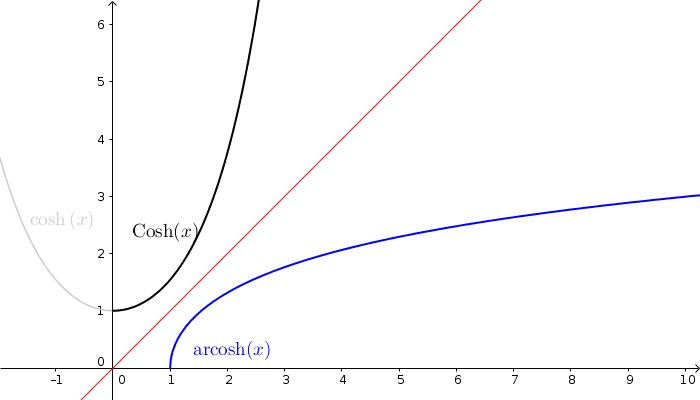
\includegraphics[width=11cm,keepaspectratio=true]{./myndir/kafli04/07_arcosh.png}
\end{center}

\subsubsection{Í framtíðinni}
Við höfum séð að veldisvísisfallið og logrinn tengjast
breiðbogaföllunum töluvert og það sama á við um hornaföllin. 
Seinna, nánar tiltekið í Stærðfræðigreiningu III, þá sjáið
þið að hornaföllin og breiðbogaföllin eru bara mismunandi hliðar
á veldisvísisfallinu.

\begin{center}
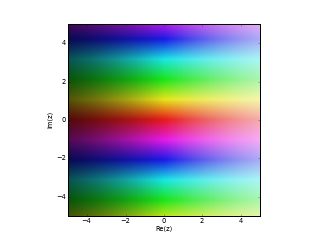
\includegraphics[width=5cm,keepaspectratio=true]{./myndir/kafli04/07_exp.png}
\end{center}
%

\end{document}
